\chapter{OpenGL applications}
\label{chap:OpenGL_app}

%\lstloadlanguages{[Visual]C++,[ISO]C++}
\lstset{language={[ISO]C++}}
\lstset{numbers=left, numberstyle=\tiny,
  stepnumber = 5, numbersep=5pt, keywordstyle=\color{blue}}

With OpenGL, you must build up your desired model from a small set of geometric
primitives (Sect.\ref{sec:primitives}) - points, lines, and polygons.
A sophisticated library that provides these features could certainly be built on top of OpenGL.
\begin{itemize}
  \item GLU - Sect.\ref{sec:glu}. GLU is a standard part of every OpenGL
  implementation
  
  \item Open Inventor: available separately for many implementations of OpenGL
\end{itemize}

OpenGL is a state machine (Sect.\ref{sec:state-mach-glen}).

Naive draw loop
\begin{lstlisting}
foreach (object) 
{
   // bind framebuffer
   
   // set depth, blending, etc. states
   
   // bind shaders
   
   // bind textures
    
   // bind vertex/index buffers
   
   WriteUniformData (object);
   glDrawElement(
       GL_TRIANGLES,
       object->indexCount,
       GL_UNSIGNED_SHORT,
       0);

}
\end{lstlisting}



\section{Client/Server}
\label{sec:clientserver}

In OpenGL's case, the client side is code that lives in the main CPU's
memory and is executed within the application program, or within the
driver in main system memory.  The rendering commands and data and
sends to the server for execution.
\begin{figure}[hbt]
  \centerline{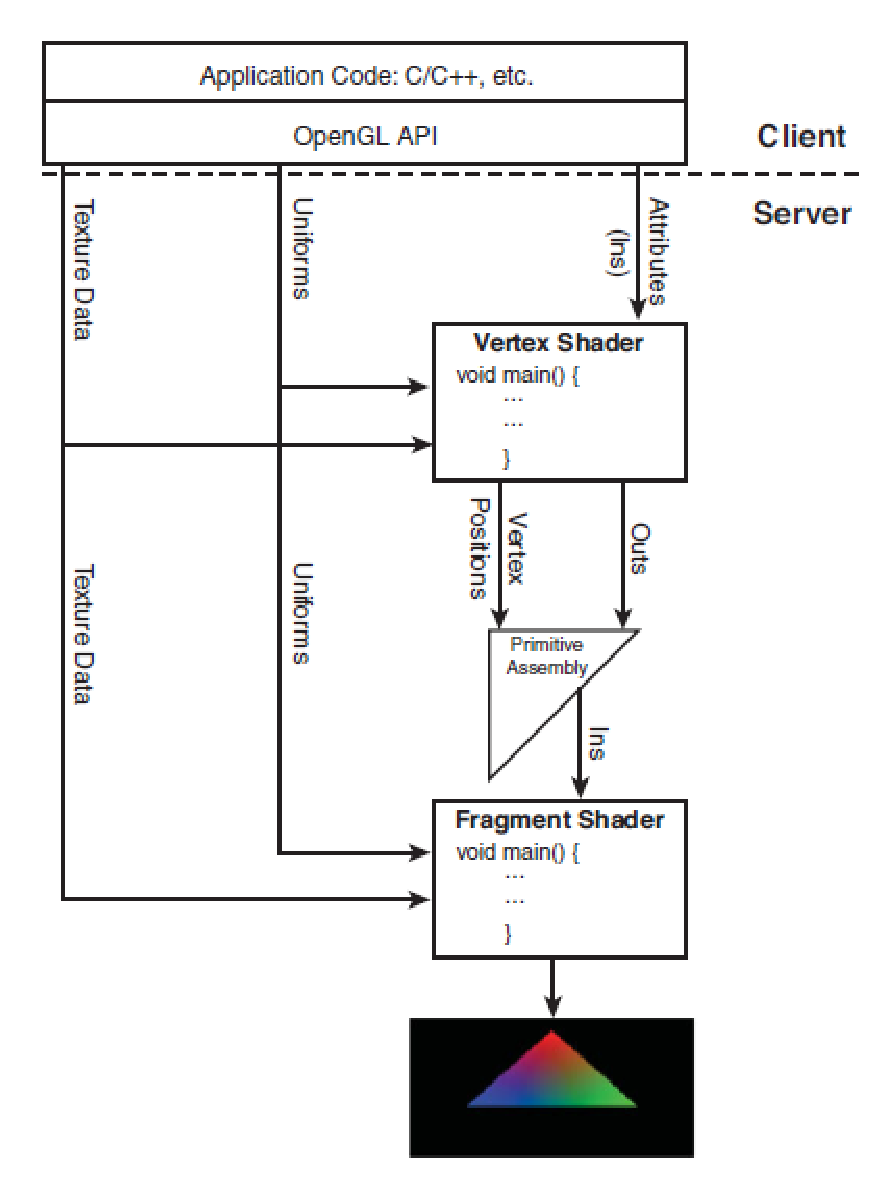
\includegraphics[height=8cm,
    angle=0]{./images/client_server.eps}}
  \caption{Steps to render a triangle}
  \label{fig:client_server}
\end{figure}

{\bf Shaders} are programs (with its own main() function) running on
server sides. There are two types: vertex shaders and fragment
shaders, Fig.~\ref{fig:client_server}. Both are written by the
language
GLSL\footnote{In general, we may have geometry shader that can
  (optionally) fit between, as well as sort of feedback mechanism for
  moving data back and forth. There can be also some post fragment
  processing features such as blending, stencil, and depth testing}.
Nowadays, we can programs shaders programs, using CUDA - a C
extension, under the name {\bf kernels} in CUDA context. We can easily
map the data from CUDA memory space to OpenGL memory space easily via
Map/Unmap mechanism (read Sect.~\ref{sec:cuda-app.-with}).

A vertex shader do the job for a single vertex (data incoming from the
client), including: applying transformations, or doing other types of
math to calculate lighting effects, displacement, color values, and so
on. To render a triangle with three vertices, the vertex shader is
executed three times, once for each vertex.

Data passed to shaders are called attributes and are composed of
\begin{enumerate}
\item vertex (location information)

\item color

\item normal (surface normal)

\item uniforms, 

\item textures.(primary + secondary)
\end{enumerate}


\subsection{Attributes (vertex, color)}
\label{sec:attributes}

An attribute is something that change per vertex. So, they can be
\begin{enumerate}
\item location (maximum 3 components) - XYZ
\item color (maximum 4 components) - RGBA
\end{enumerate}
Attributes can be floating-point, integer, or boolean data, and
attributes are always stored internally as a four component vector,
even if you don't use all four components.

% Attributes, however, can have any meaning you want in the vertex
% program; you are in control.


\begin{framed}
  Attributes are copied from a pointer to local client memory to a
  buffer that is stored (most likely) on the graphics
  hardware. Attributes are only processed by the vertex shader (read
  Sect.~\ref{sec:shaders}) and have no meaning to the fragment shader.
\end{framed}

Everything starts with the atoms ``vertex''. Each vertex can have some
attributes (maximum 16, numbered from 0 to 15 and can be assigned to
any variable in the shader program). 

\begin{table}[hbt]
  \begin{center}
    \caption{Predefined attribute identifiers}
    \begin{tabular}{cp{8cm}} 
      \hline
      Identifier & Description \\
      \verb!GLT_ATTRIBUTE_VERTEX! & Three component (x, y, z) vertex position\\
      \verb!GLT_ATTRIBUTE_COLOR! & Four component (r, g, b, a) color value\\
      \verb!GLT_ATTRIBUTE_NORMAL! & Three components (x, y, z) surface
      normal \\
      \verb!GLT_ATTRIBUTE_TEXTURE0! & Primary two component (s, t) texture
      coordinate \\
      \verb!GLT_ATTRIBUTE_TEXTURE1! & Secondary two component (s, t) texture
      coordinate \\
      \hline\hline
    \end{tabular}
  \end{center}
  \label{tab:attribute_id}
\end{table}

% \begin{verbatim}
% GLT_ATTRIBUTE_VERTEX
% GLT_ATTRIBUTE_COLOR 
% GLT_ATTRIBUTE_NORMAL 
% GLT_ATTRIBUTE_TEXTURE0
% GLT_ATTRIBUTE_TEXTURE1 
% \end{verbatim}

\subsection{Uniforms}
\label{sec:uniforms}

A uniform is a single value that doesn't change for the entire batch
attributes. Uniforms can be used for virtually an unlimited number of
uses.

\begin{itemize}
\item set a single color value that is applied to an entire surface. 
\item set a time value that you change every time you render to do
  some type of vertex animation (note the uniform changes once per
  batch, not once per vertex here).

\item One of the most common uses of uniforms is to set transformation
  matrices in the vertex shader (this is almost the entire purpose
\end{itemize}
Like attributes, uniform values can be floating-point, integer, or
boolean in nature, but unlike attributes, you can have uniform
variables in both the vertex and the fragment shader.

\begin{framed}
  Uniforms can be scalar or vector types, and you can have matrix uniforms.
\end{framed}


\subsection{Textures}
\label{sec:textures}

Texture values can be sampled and filtered from both the vertex shader
and the fragment shader.  Fragment shaders typically sample a texture
to apply image data across the surface of a triangle.

Texture data, however, is more useful than just to represent
images. Most image file formats store color components in unsigned
byte values (8 bits per color channel), but you can also have
floating-point textures. This means potentially any large block of
floating- point data, such as a large lookup table of an expensive
function, could be passed to a shader in this way.

We will learn more in Sect.~\ref{sec:arrays-=-textures}. 
% \section{Vertex}
% \label{sec:vertex}



\section{State machine (glEnable/glDisable)}
\label{sec:state-mach-glen}

You put it into various states (or modes) that then remain in effect until you
change them. As you've already seen, the current color is a state variable. 

For a given piece of geometry, there are many things that can affect
how it is drawn, e.g. 
\begin{itemize}
\item is the object blended in the background?
\item are we performing front or back face culling?
\item ...
\end{itemize}
The collection of all of these parameters is called a {\bf state} of
the pipeline. So, OpenGL works as a state machine. The state variables
in general can have more than 2 values.

\url{http://www.glprogramming.com/red/chapter01.html}

For those that receives one of two possible values only, they are
associated with turn on or off. So, OpenGL provides 2 functions to do
this: \verb!glEnable/glDisable!.
\begin{verbatim}
void glEnable(GLenum capability);

void glDisable(GLenum capability);

GLboolean glIsEnabled(GLenum capability);
\end{verbatim}


E.g.: depth testing if enabled, will force OpenGL to check to make
sure the object is in front of other things behind it, before being
rendered. 
\begin{verbatim}
glEnable(GL_DEPTH_TEST);
\end{verbatim}


For those that can receive more than 2 values. A set of query
functions allows you to query the values of Booleans, integers,
floats, and double variables. These four functions are prototyped
thus:
\begin{verbatim}
void glGetBooleanv(GLenum pname, GLboolean *params);
void glGetDoublev(GLenum pname, GLdouble *params);
void glGetFloatv(GLenum pname, GLfloat *params);
void glGetIntegerv(GLenum pname, GLint *params);
\end{verbatim}
Each function returns a single value or a whole array of values,
storing the results at the address you supply.



\section{Intermediate mode vs. Vertex Arrays vs. Display List}
\label{sec:interm-mode-vs}

This section describes different programming approaches used in
OpenGL. 

\subsection{Intermediate mode}
\label{sec:intermediate-mode-1}

{\bf Intermediate-Mode is the firs approach}, used in OpenGL 1.0. In
this mode, all rendering functions are called between
\verb!glBegin/glEnd!. So, it requires explicit functional calls to
draw every geometric primitive shapes. They can be

\begin{enumerate}
\item \verb!glVertex[size][type]v! : call this OpenGL API to specify
  the location of the vertex (2D or 3D ...)

  with \verb!size! is 2, 3 or 4; \verb!type! is any of [s,i,f,d]
  (corresponding to short, int, float, and double). 

\item For other types of arrays, we have similar syntax,
  e.g. \verb!glColor[size][type]v!, \verb!glNormal[size][type]v!...
\end{enumerate}

However, this approach would be come slow for complex geometric
primitive composed of thousands of vertex due to thousands of
functional calls and many of them are redundant. Another factor that
slow down the performance is that data need to be transferred so often
from CPU RAM to GPU RAM. 

\subsection{Vertex Arrays}
\label{sec:vertex-arrays}

To resolve the first problem, i.e. functional call redundancy, OpenGL
1.1 introduced vertex data into arrays, and then use blocks of data in
these arrays to specify the multiple geometric primitives through the
execution of a single command.
\begin{verbatim}
  // Setup a triangle
  // Here, we use vertex array, i.e. every triple form a vertex
  GLfloat vVerts[] = { -0.5f, 0.0f, 0.0f,
                    0.5f, 0.0f, 0.0f,
                    0.0f, 0.5f, 0.0f };
\end{verbatim}
which we use to 
\begin{verbatim}
  // create a Vertex Array object
  glGenBuffers(1, &uiVertexArray);
  // bind to ARRAY BUFFER
  glBindBuffer(GL_ARRAY_BUFFER, uiVertexArray);
  // finally, add data to it
  glBufferData(GL_ARRAY_BUFFER, sizeof(GLfloat) * 3 * nNumVerts, 
               vVerts, GL_DYNAMIC_DRAW);
\end{verbatim}
In complicated case, we can check
\begin{verbatim}
  // First time, create the buffer object, allocate the space
  if(uiVertexArray == 0) {
        glGenBuffers(1, &uiVertexArray);
        glBindBuffer(GL_ARRAY_BUFFER, uiVertexArray);
        glBufferData(GL_ARRAY_BUFFER, 
              sizeof(GLfloat) * 3 * nNumVerts, 
              vVerts, GL_DYNAMIC_DRAW);
        }
  else        { // Just bind to existing object
        glBindBuffer(GL_ARRAY_BUFFER, uiVertexArray);

        // Copy the data in
        glBufferSubData(GL_ARRAY_BUFFER, 0, 
                  sizeof(GLfloat) * 3 * nNumVerts, vVerts);
        pVerts = NULL;
        }
  }
\end{verbatim}

\textcolor{red}{We can use up to 6 arrays: corresponding to arrays of
  vertices, normals, colors components, color indices, texture
  coordinates, Boolean edge flags}.
We use the following 6 functions to specify the location, and data
format of the corresponding type of
array\footnote{\url{http://personal.redestb.es/jmovill/opengl/openglonwin-15.html}}.

\begin{verbatim}
glVertexPointer(int size, enum type, sizei stride, void *pointer)
glNormalPointer(...)
glColorPointer
glIndexPointer
glTexCoordPointer
glEdgeFlagPointer
\end{verbatim}
with (suppose Vertex Array)
\begin{enumerate}
\item \verb!size! = number of coordinates per vertex (e.g. with 3D
  vertex, size = 3)
\item \verb!type! = data type for each coordinate
  (\verb!GL_SHORT, GL_INT!, \verb!GL_FLOAT, or GL_DOUBLE!)

  Other array types may use different data type, e.g. Boolean edge
  flags only use \verb!GL_BOOL!
\begin{verbatim}
glVertexPointer   2,3,4   short, int, float, double
glNormalPointer   3       byte, short, int, float, double
glColorPointer 	  3,4     byte, ubyte, short, ushort, int,  
                          uint, float, double 
glIndexPointer    1       ubyte, short, int, float, double
glTexCoordPointer 1,2,3,4 short, int, float, double
glEdgeFlagPointer 1       boolean
\end{verbatim}

\item \verb!stride! = byte offset between pointers to consecutive
  vertexes (if stride = 0, the vertex data are tightly packed)
\item \verb!pointer! = the pointer pointing to the first coordinate of
  the first vertex in the array. 
\end{enumerate}

\begin{framed}
  Data components within an array element are stored
  sequentially. Array elements can be non-contiguous, i.e. when stride
  $.ne.$ 0. If stride = 0, then array elements are stored sequentially
  as well. 
\end{framed}

% gl[...]Pointer: OpenGL give 6 different pointers when using
% glDrawArrays/Elements. The most commonly use function is
% \verb!glVertexPointer()!.

These data reside on client-side, and are disabled by default. So, we
need to enable which one we want to use using
\verb!glEnableClientState(enum array)! and
\verb!glDisableClientState(..)!  with \verb!array! token can be.
\begin{verbatim}
GL_VERTEX_ARRAY
GL_NORMAL_ARRAY
GL_COLOR_ARRAY
GL_INDEX_ARRAY
GL_TEXTURE_COORD_ARRAY
GL_EDGE_FLAG_ARRAY
\end{verbatim}

\begin{framed}
  We generally discuss Vertex Array, as other type of arrays mainly
  provide accompanying information to the Vertex Array and most of the
  time we work with Vertex Array data.

  \textcolor{red}{Like intermediate-mode, the data in Vertex Arrays
    reside in CPU RAM, and need to move to server-side memory (i.e. GPU
    DRAM) every time rendering is required}.
\end{framed}


To render data using Vertex Arrays, new OpenGL APIs are provided and
used between \verb!glBegin/glEnd!

\begin{enumerate}
\item \verb!glArrayElement(int i )!: transfer (i.e. draw) the element
  $i$-th to OpenGL (i.e. GPU memory), i.e. draw points from a single
  array.

\item \verb!glDrawArrays!: (combine array elements from different
  enabled arrays) for each enabled array, we construct a sequence of
  geometric primitives using array elements from \verb!first! through
  \verb!count! of each enabled array.
\begin{verbatim}
void glDrawArrays ( enum mode, int first, sizei count ) ;
\end{verbatim}
  with \verb!mode! tell which kind of primitive to construct (the same
  token passing to \verb!glBegin()!. 

  So, we don't need to work with individual vertexes, OpenGL will
  automatically iterate through array elements and do the work

\item \verb!glDrawElements()!: (combine continuous array elements from
  a single array) we iterate through array elements in the array
  specified by \verb!indices! and call \verb!glArrayElement()! for
  each element until it reaches \verb!count! element count.
\begin{verbatim}
void glDrawElements ( enum mode, sizei count, 
                 enum type, void *indices );
\end{verbatim}
  with \verb!mode!, again, is the type of geometric primitive to
  construct. 

\item \verb!glInterleavedArrays!: (combine interleaved elements from a
  single array) allow sending vertices data to the graphics card using
  a single array
\begin{verbatim}
void glInterleavedArrays ( enum format, sizei stride, void *pointer )
\end{verbatim}

\item If any of the arrays other Vertex Arrays are enabled, they are
  indeterminate after the execution of glDrawElements(), otherwise,
  the values are unchanged. 
\end{enumerate}

As a result, with the OpenGL 1.1 (array-based) approach, you would
transfer your few hundred KB of vertex data across the bus every time
you wanted to render a model. This meant that you could modify your
array-based data in memory as the next time you sent it the new data
would be transferred. Compared to (static) display lists, this made
array-based data the natural choice for frequently updated geometry.


Summary of new functions in OpenGL 1.1.
\begin{verbatim}
glArrayElement(), glDrawArrays(), glVertexPointer(), 
glNormalPointer(), glColorPointer(), glIndexPointer(), 
glTexCoordPointer(), glEdgeFlagPointer(), glGetPointerv(), 
glDrawElements(), glInterleavedArrays().
\end{verbatim}

An example is given in Sect.~\ref{sec:example-fortr-freegl-1}. 

\subsection{Display List}
\label{sec:display-list}


{\bf Display List} is a list of OpenGL commands that are executed only
once and the result are stored on the server side, i.e. GPU. After the
display list has been compiled and executed, we can reuse the result
as many time as we want without re-evaluating nor re-transmitting from
client (CPU) to server (GPU). However, they cannot be modified. So,
this method is best for static data.
\textcolor{red}{If we want the data to reside on graphics card memory
  and the data, however, change quite often, it's better to consider
  VBO}.

Data in display list can also be shared by many clients.Since display
list is a part of server state, any client commands cannot be used.
\begin{verbatim}
glFlush(), glFinish(), glRenderMode(), 
glEnableClientState(), glVertexPointer(), etc. 
\end{verbatim}
The same to OpenGL commands that return a value, as the value is
returned to the client side.
\begin{verbatim}
glIsEnabled(), glGet*(), glReadPixels(), 
glFeedbackBuffer(), etc.
\end{verbatim}

How to use display list?
\begin{enumerate}
\item \verb!glGenLists(int num)!: (optional) create one or more
  continuous display list objects. Return 0 if errors occur.

\item Commands in the display lists are between \verb!glNewList()! and
  \verb!glEndList()!, prior to rendering. 
\begin{verbatim}
glNewList(dListID, mode)
...
glEndList()
\end{verbatim}
  with \verb!mode! can be \verb!GL_COMPILE! (compile only),
  \verb!GL_COMPILE_AND_EXECUTE! (compile and then render).

\item Now, to invoke one or more display lists, we use
  \verb!glCallList(dListID)! or \verb!glCallLists()! every frame. We
  put this inside the callback.
\end{enumerate}

\begin{verbatim}
// create one display list
GLuint index = glGenLists(1);

// compile the display list, store a triangle in it
glNewList(index, GL_COMPILE);
    glBegin(GL_TRIANGLES);
    glVertex3fv(v0);
    glVertex3fv(v1);
    glVertex3fv(v2);
    glEnd();
glEndList();
...

// draw the display list
glCallList(index);
...

glCallList(index); //call again (data is now stored in 
                   //server-side, very fast)

// delete it if it is not used any more
glDeleteLists(index, 1);
\end{verbatim}

For example, read Sect.~\ref{sec:example-fortran-glut}.

References:
\begin{itemize}
\item \url{http://www.songho.ca/opengl/gl_displaylist.html}
\end{itemize}


\section{Graphics effects}
\label{sec:graphics-effects}

\subsection{Face culling}
\label{sec:face-culling}

By default, every point, line, or triangle you render is rasterized
on-screen and in the order in which you specify when you assemble the
primitive batch. One problem that can occur is if you draw a solid
object made up of many triangles, the triangles drawn first can be
drawn over by triangles drawn afterward. 

The {\it painter algorithm} draw the farther triangles first, and the
nearer later. However, this is inefficient. A better solution is {\bf
  face culling}. 

Culling away the front of solid geometry is also useful in some
circumstances, for example, showing a rendering of the insides of some
figure. When rendering transparent objects (blending is coming up
soon), we often render an object twice, once with transparency on,
culling the front sides, and then again with the back sides turned
off. This layers the object with the back side rendered before the
front side, a requirement for rendering things transparently.

General face culling is turned on/off like this:
\begin{verbatim}
glEnable(GL_CULL_FACE);

glDisable(GL_CULL_FACE);
\end{verbatim}

Note, we did not say whether to cull the front or back of
anything. That is controlled by another function, glCullFace.
\begin{verbatim}
void glCullFace(GLenum mode);
\end{verbatim}
Valid values for the mode parameter are \verb!GL_FRONT!,
\verb!GL_BACK!, or \verb!GL_FRONT_AND_BACK!. To throw away the insides
of opaque (nontransparent) geometry takes two lines of code then.
\begin{verbatim}
glCullFace(GL_BACK);
glEnable(GL_CULL_FACE);
\end{verbatim}
Back face culling can significantly improve performance and corrects
some problems.

\subsection{Depth testing}
\label{sec:depth-testing}

Another technique for hidden surface removal is called depth
testing. The idea is that when a vertex is drawn, it is assigned a
depth value (z value) that denotes its distance from the viewer's
perspective. Next time, when another vertex is drawn at that location,
it's z value will be used to compared with the current pixel. If the
value is higher, it's closer to the viewer, so the old value of the
pixel is overwritten by this new value. 

Using depth testing is recommended
\begin{verbatim}
glutInitDisplayMode(GLUT_DOUBLE | GLUT_RGBA | GLUT_DEPTH);

glEnable(GL_DEPTH_TEST);
\end{verbatim}

\subsection{Polygon modes}
\label{sec:polygon-modes}

By default, any polygon (triangles, quad, ...) are drawn as
solid. However, you can change the setting (e.g. draw wireframe) using
\begin{verbatim}
void glPolygonMode(GLenum face, GLenum mode);
\end{verbatim}
Like in face culling, the face parameter can be 
\begin{verbatim}
GL_FRONT, GL_BACK, or GL_FRONT_AND_BACK.
\end{verbatim}
The mode parameter can be \verb!GL_FILL! (the default),
\verb!GL_LINE!, or \verb!GL_POINT!. 

\subsection{Polygon offsets}
\label{sec:polygon-offsets}

Sometimes, you want two polygon modes, Fig.~\ref{fig:polygon_offset}

\begin{figure}[hbt]
  \centerline{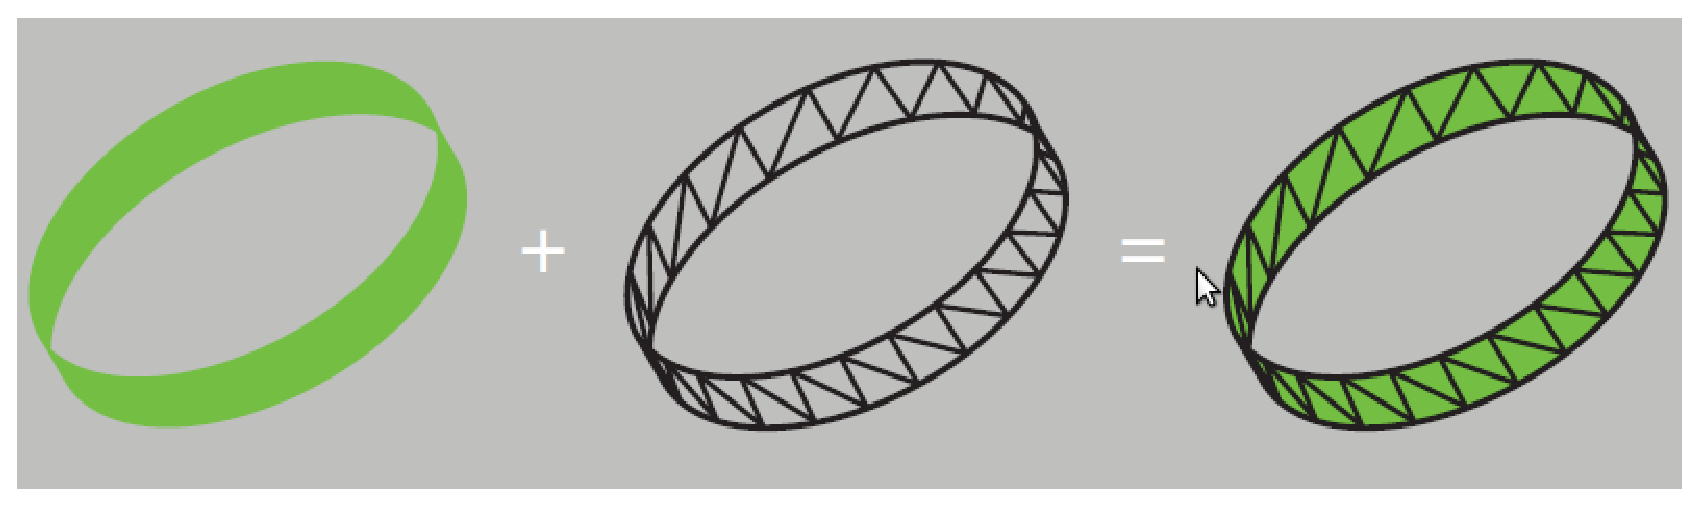
\includegraphics[height=3cm,
    angle=0]{./images/polygon_offset.eps}}
  \caption{When you want both solid and wireframe drawings}
  \label{fig:polygon_offset}
\end{figure}


\subsection{Scissors }
\label{sec:scissors-}

If you know the exact region that need to redrawn, you can explicitly
tell OpenGL to redraw that region only. This can help improve the
performance as the system doesn't have to re-draw all. This is known
as scissor test.

\begin{verbatim}
glEnable(GL_SCISSOR_TEST);

// tell the rectangle
void glScissor(GLint x, GLint y, GLsizei width, GLsizei height);
\end{verbatim}
after that, you can turn off that scissor test.


This is the sample callback
\begin{verbatim}
void RenderScene(void)
{
  // Clear blue window
  glClearColor(0.0f, 0.0f, 1.0f, 0.0f);
  glClear(GL_COLOR_BUFFER_BIT);

// Now set scissor to smaller red sub region
  glClearColor(1.0f, 0.0f, 0.0f, 0.0f);
  glScissor(100, 100, 600, 400);
  glEnable(GL_SCISSOR_TEST);
  glClear(GL_COLOR_BUFFER_BIT);

// Finally, an even smaller green rectangle
glClearColor(0.0f, 1.0f, 0.0f, 0.0f);
glScissor(200, 200, 400, 200);
glClear(GL_COLOR_BUFFER_BIT);

// Turn scissor back off for next render
  glDisable(GL_SCISSOR_TEST);
  
  glutSwapBuffers();
}
\end{verbatim}

\subsection{Blending}
\label{sec:blending}

Blending is a intermediate mode between DEPTH testing ON and OFF. It
means that the color value of the two (or more) vertices at the same
pixel are combined to create the blending effect.

\begin{verbatim}
glEnable(GL_BLEND);
\end{verbatim}

By default, the combined color use the formula (you can change the equation)
\begin{verbatim}
Cf = (Cs * S) + (Cd * D)

Cs  = source color
Cd  = destination color
Cf  = combined color
\end{verbatim}
with S and D are blending factors, given to OpenGl via
\begin{verbatim}
glBlendFunc(GLenum S, GLenum D);
\end{verbatim}
which can be any of the following value,
Table~\ref{tab:blending_factor}. The constant blending factor is
initially black (0.0f, 0.0f, 0.0f, 0.0f), but it can be changed with
this function:
\begin{verbatim}
void glBlendColor(GLclampf red, GLclampf green, 
                  Glclampf blue,
                  GLclampf alpha);
\end{verbatim}

\begin{verbatim}
GLfloat vRed[] = { 1.0f, 0.0f, 0.0f, 0.5f };
glEnable(GL_BLEND);
glBlendFunc(GL_SRC_ALPHA, GL_ONE_MINUS_SRC_ALPHA);
shaderManager.UseStockShader(GLT_SHADER_IDENTITY, vRed);
squareBatch.Draw();
glDisable(GL_BLEND);
\end{verbatim}

\begin{table}[hbt]
  \begin{center}
    \caption{OpenGL blending factor, $f = min(As, 1-Ad)$}
    \begin{tabular}{ccc} 
      \hline
      Function & RGB Blend Factors & Factor \\
      \verb!GL_ZERO! & (0,0,0) &  0 \\
      \verb!GL_ONE!& (1,1,1) & 1 \\
      \verb!GL_SRC_COLOR! & (Rs,Gs,Bs) & As \\
      \verb!GL_ONE_MINUS_SRC_COLOR! & (1,1,1) - (Rs,Gs,Bs) & 1 - As \\
      \verb!GL_DST_COLOR! & (Rd,Gd,Bd) & Ad \\
      \verb!GL_ONE_MINUS_DST_COLOR! & (1,1,1) - (Rd,Gd,Bd) & 1 - Ad \\
      \verb!GL_SRC_ALPHA! & (As,As,As) & As \\
      \verb!GL_ONE_MINUS_SRC_ALPHA! & (1,1,1) - (As,As,As) & 1 - As \\
      \verb!GL_DST_ALPHA! & (Ad,Ad,Ad) & Ad \\
      \verb!GL_ONE_MINUS_DST_ALPHA! & (1,1,1) - (Ad,Ad,Ad) & 1 - Ad  \\
      \verb!GL_CONSTANT_COLOR! & (Rc,Gc,Bc) & Ac \\
      \verb!GL_ONE_MINUS_CONSTANT_COLOR! & (1,1,1) - (Rc,Gc,Bc) & 1 - Ac \\
      \verb!GL_CONSTANT_ALPHA! & (Ac,Ac,Ac) & Ac \\
      \verb!GL_ONE_MINUS_CONSTANT_ALPHA! & (1,1,1) - (Ac,Ac,Ac) & 1 - Ac \\
      \verb!GL_SRC_ALPHA_SATURATE! & (f,f,f)* & 1 \\
      \hline\hline
    \end{tabular}
  \end{center}
  \label{tab:blending_factor}
\end{table}

You can change the equation using
\begin{verbatim}
void glBlendEquation(GLenum mode);
\end{verbatim}
with mode is given in Table~\ref{tab:blending_equation}. Or you can
give your own equation for RGB and another for Alpha channel.
\begin{verbatim}
void glBlendFuncSeparate(GLenum srcRGB, GLenum dstRGB, 
              GLenum srcAlpha, 
              GLenum dstAlpha);
\end{verbatim}


\begin{table}[hbt]
  \begin{center}
    \caption{Blending formula}
    \begin{tabular}{cc} 
      \hline
      Mode & Function \\
      \verb!GL_FUNC_ADD! (default) & Cf = (Cs * S) + (Cd * D) \\
      \verb!GL_FUNC_SUBTRACT! & Cf = (Cs * S) - (Cd * D) \\
      \verb!GL_FUNC_REVERSE_SUBTRACT! & Cf = (Cd * D) - (Cs * S) \\
      \verb!GL_MIN! & Cf = min(Cs, Cd) \\
      \verb!GL_MAX! & Cf = max(Cs, Cd) \\
      \hline\hline
    \end{tabular}
  \end{center}
  \label{tab:blending_equation}
\end{table}

\subsection{Anti-aliasing}
\label{sec:anti-aliasing}

First
\begin{verbatim}
// blend equation is set to GL_ADD
// then
glEnable(GL_BLEND);
glBlendFunc(GL_SRC_ALPHA, GL_ONE_MINUS_SRC_ALPHA);
\end{verbatim}
Then you can choose
\begin{verbatim}
glEnable(GL_POINT_SMOOTH); // Smooth out points
glEnable(GL_LINE_SMOOTH); // Smooth out lines
glEnable(GL_POLYGON_SMOOTH); // Smooth out polygon edges
\end{verbatim}
One of the biggest advantages to antialiasing is that it smoothes out
the edges of primitives and can lend a more natural and realistic
appearance to renderings. \textcolor{red}{Point and line smoothing is widely
  supported, but unfortunately polygon smoothing is not available on all
  platforms (even the mode is there)}. Modern feature to polygon
smoothing is multisampling (next section). 



You can create a function to switch between On/Off anti-aliasing
\begin{verbatim}
///////////////////////////////////////////////////////////////////////
// Reset flags as appropriate in response to menu selections
void ProcessMenu(int value)
{
  switch(value)
  {
   case 1:
// Turn on antialiasing, and give hint to do the best
// job possible.
     glBlendFunc(GL_SRC_ALPHA, GL_ONE_MINUS_SRC_ALPHA);
     glEnable(GL_BLEND);
     glEnable(GL_POINT_SMOOTH);
     glHint(GL_POINT_SMOOTH_HINT, GL_NICEST);
     glEnable(GL_LINE_SMOOTH);
     glHint(GL_LINE_SMOOTH_HINT, GL_NICEST);
     glEnable(GL_POLYGON_SMOOTH);
     glHint(GL_POLYGON_SMOOTH_HINT, GL_NICEST);
   break;
   case 2:
// Turn off blending and all smoothing
     glDisable(GL_BLEND);
     glDisable(GL_LINE_SMOOTH);
     glDisable(GL_POINT_SMOOTH);
     glDisable(GL_POLYGON_SMOOTH);
     break;
     default:
   break;
   }
// Trigger a redraw
  glutPostRedisplay();
}
\end{verbatim}

\subsection{Multi-sampling}
\label{sec:multi-sampling}

All primitives are sampled multiple times per pixel, and the results
are stored in this buffer. These samples are resolved to a single
value each time the pixel is updated, so from the programmer's
standpoint, it appears automatic and happens 'behind the scenes'.

\begin{verbatim}
glutInitDisplayMode(GLUT_DOUBLE | GLUT_RGB | GLUT_DEPTH | GLUT_MULTISAMPLE);
\end{verbatim}

You should use this for polygons only. So, make sure you disable that
when draw points or lines
\begin{verbatim}
glDisable(GL_MULTISAMPLE);
glEnable(GL_POINT_SMOOTH);
// Draw some smooth points
// ...
glDisable(GL_POINT_SMOOTH);
glEnable(GL_MULTISAMPLE);
\end{verbatim}


The multisample buffers use the RGB values of fragments by default and
do not include the alpha component of the colors. You can change this
by calling glEnable with one of the following three values:
\begin{verbatim}
GL_SAMPLE_ALPHA_TO_COVERAGE  Use the alpha value.
GL_SAMPLE_ALPHA_TO_ONE Set alpha to 1 and use it.
GL_SAMPLE_COVERAGE   Use the value set with glSampleCoverage.
\end{verbatim}
When \verb!GL_SAMPLE_COVERAGE! is enabled, the glSampleCoverage
function allows you to specify a value that is ANDed (bitwise) with
the fragment coverage value: void glSampleCoverage(GLclampf value,
GLboolean invert);



\section{Example}
\label{sec:example-1}

% \subsection{A window}
% \label{sec:window}



\subsection{Intermediate mode - drawing primitives}
\label{sec:intermediate-mode}

\url{http://nehe.gamedev.net/data/lessons/lesson.asp?lesson=02}

OpenGL is a state-based system, and any parameters that you set is
sticky, i.e. it remains the same until you change it. Modes and
attributes are enabled/disabled using \verb!glEnable/glDisable!. We
can check a state is currently enabled or not using
\verb!glIsEnabled()!. State variables can be saved into the
stack/restored using \verb!glPushAttrib/glPopAttrib!. The number of
stacks must be at least 16 in OpenGL standard (check with
\verb!glInfo()!).
\begin{verbatim}
glPushAttrib(GL_LIGHTING_BIT);    // elegant way to change states because
   glDisable(GL_LIGHTING);       // you can restore exact previous states
   glEnable(GL_COLOR_MATERIAL);  // after calling glPopAttrib()

glPushAttrib(GL_COLOR_BUFFER_BIT);
   glDisable(GL_DITHER);
   glEnable(GL_BLEND);

... // do something

glPopAttrib();                    // restore GL_COLOR_BUFFER_BIT
glPopAttrib();                    // restore GL_LIGHTING_BIT
\end{verbatim}


The example below is to draw an a rectangle primitive (i.e. the Quad),
then add a texture on it. The texture can be an image, a color pattern
.... Suppose the resource to the texture is reference via the variable
\verb!textureID!.

\begin{lstlisting}
glBindTexture( GL_TEXTURE_2D, textureID);

glColor3f(1.0f, 0, 0);
 // I want to start drawing a QUAD, i.e. OpenGL will automatically
 // connect the 4 vertices with coordinates provided
glBegin(GL_QUADS);
  glTexCoord2i (0, h);
  glVertex3f(0, 0, 0);

  glTexCoord2i(0, 0); 
  glVertex3f(0, 1.0f, 0);
 
  glTexCoord2i(w, 0);
  glVertex3f(1.0f, 1.0f, 0);

  glTexCoord2i(w, h);
  glVertex3f(1.0f, 0, 0);
glEnd();

 // add texture here
 // ...
   
 // use double buffer mechanism
SwapBuffers(hDC);
\end{lstlisting}

The order of the vertices is
\begin{verbatim}
   v1 - - - -v4            v1
   |         |            / \
   |         |           /   \
   v2 - - - -v3         v2---v3
\end{verbatim}


Traditionally, to draw a primitive (points, lines, triangles,
polygons) in OpenGL, we need to put the functional calls between
\verb!glBegin/glEnd!. This is known as {\bf intermediate mode}. For a
list of primitives, read Sect.~\ref{sec:primitives}. If we want to
draw a series of 4 quads, we just put 4 groups of functional calls
like above between a single pair of \verb!glBegin/glEnd!. 

Another example is to draw a cube using intermediate approach. As cube
is not a primitives, we need to build them from 6 Quads.
\begin{verbatim}
glBegin(GL_QUADS);      // draw a cube with 6 quads
    glVertex3fv(v0);    // front face
    glVertex3fv(v1);
    glVertex3fv(v2);
    glVertex3fv(v3);

    glVertex3fv(v0);    // right face
    glVertex3fv(v3);
    glVertex3fv(v4);
    glVertex3fv(v5);

    glVertex3fv(v0);    // up face
    glVertex3fv(v5);
    glVertex3fv(v6);
    glVertex3fv(v1);

    ...                 // draw other 3 faces

glEnd();
\end{verbatim}
With 6 faces, Fig.~\ref{fig:cube}, we need 24 glVertex*() calls. If we
need to color or normal the object, we may need 3 times more calls to
glColor*() and glNormal*(). In this example, a single vertex is
redundantly called three times.

\begin{figure}[hbt]
  \centerline{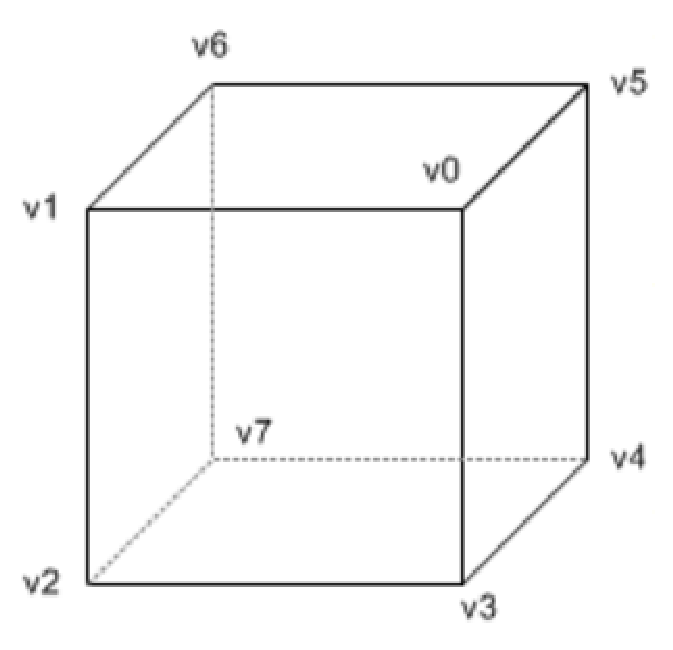
\includegraphics[height=5cm,
    angle=0]{./images/cube.eps}}
\caption{A cube with 6 vertices}
\label{fig:cube}
\end{figure}


As you can see, in intermediate mode, we need to call functions to set
the data for every vertex. For a geometric shape with thousands of
primitives, a better way is to use Vertex Arrays (read
Sect.~\ref{sec:cuda-app.-with}). 

\begin{framed}
  Note that not all of OpenGL commands can be placed in between
  glBegin() and glEnd(). Only a subset of commands can be used;
  glVertex*(), glColor*(), glNormal*(), glTexCoord*(), glMaterial*(),
  glCallList(), etc.

  To work with Vertex Arrays, OpenGL provides 3 new functions:
  glDrawArrays(), glDrawElements(), and
  glDrawRangeElements(). Although, an even better approach is using
  Vertex Buffer Objects (VBO) or Displayed
  List\footnote{\url{http://www.songho.ca/opengl/gl_displaylist.html}}.  
\end{framed}

Similar to normal I/O, OpenGL commands are not executed
immediately. They are put to the buffer and executed until buffer is
full\footnote{\url{1http://www.songho.ca/opengl/gl_overview.html}}.
\verb!glFlush/glFinish! are two functions we use to flush data in
buffer to terminal.

More advanced and practical examples, please read
Sect.~\ref{sec:example-2} (GLUT/FreeGLUT),
Sect.~\ref{sec:cuda-app.-with} (CUDA-OpenGL).


References:
\begin{enumerate}
\item \url{http://www.seas.upenn.edu/~cis565/fbo.htm}
\item 
\end{enumerate}



\section{Techniques}

Techniques
\begin{enumerate}
  \item Persistent-mapped buffers
  
  faster streaming of dynamic geometry
  
  \item MultiDrawIndirect (MDI)
  
  faster submission of multiple draw calls
  
  \item Packing 2D textures into arrays
  
  texture changes no longer break batches
\end{enumerate}

